
\documentclass[paper=a4]{article}

\usepackage[left=4.5cm, right=4.5cm, top=1cm, bottom=3.2cm
  %,showframe% <- only to show the page layout
]{geometry}

\addtolength{\parskip}{\baselineskip} 
\parindent 0pt

\usepackage{graphicx}
\usepackage{config}

\usepackage{authblk}

\renewcommand\Affilfont{\fontsize{9}{10.8}\itshape}

\title{Non-random network connectivity comes in pairs}
\date{}
\author[1,2]{Felix Z.~Hoffmann}
\author[1]{Jochen Triesch}

\affil[1]{Frankfurt Institute for Advanced Studies (FIAS), Johann Wolfgang Goethe University, Frankfurt am Main, Germany}
\affil[2]{International Max Planck Research School for Neural Circuits, Max Planck Institute for Brain Research, Frankfurt am Main, Germany}

\renewcommand\Authands{ and }



\begin{document}

\pagenumbering{gobble}

\maketitle

%% \begin{center}
%% {\Large{\textbf{ Non-random network connectivity comes in pairs }}}

%% %(connection probablities that are symmetric in pairs)
%% \end{center}
%% \centerline{}
%% \centerline{Felix Z.~Hoffmann, Jochen Triesch}

Overrepresentation of bidirectional connections in local cortical networks has been repeatedly reported and is in the focus of the ongoing discussion of non-random connectivity. Here we show in a brief mathematical analysis that in a network in which connection probabilities are symmetric in pairs, $P_{ij} = P_{ji}$, the occurrence of bidirectional connections and non-random structures are inherently linked; an overabundance of reciprocally connected pairs emerges necessarily when the network structure deviates from a random network in any form. For two distributions of connection probabilities, the discrete two-point distribution and continuous gamma distribution, we quantify how a more organized structure increases reciprocity in the network.

\vspace{1cm}

\begin{figure}[h!]
  \centering
  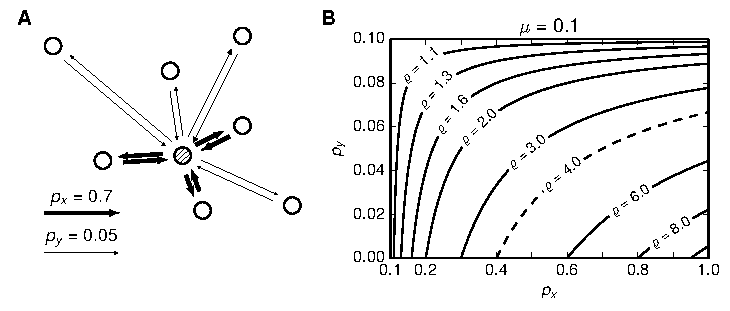
\includegraphics[width=\textwidth]{%
    ../figures/two_point_full/pub/two_point_full_pxpy.pdf} %
  \caption{Relative overrepresentation $\varrho$ of bidirectional connections in networks with a fraction of pairs connected with a high probability $p_x$ and the rest of the pairs connected with a low probability $p_y$.}
\end{figure}

\section*{Acknowledgements}

\nocite{Song2005, Perin2011, Jensen1906}

\printbibliography

\end{document}
